\section{Container and Collections}
\begin{description}
  \item[Container] Contains objects with value (vector, string, set, map)
  \item[Collection] Contains objects by reference
\end{description}

\begin{itemize}
  \itemsep -0.5em 
  \item Container can be copied easily using the constructor (deep copy). \lstinline[language=C++]|std::vector<int> vv{};|
  \item Container support the "clear()" function which empty the container.
  \item There are three types of containers: Sequence Containers, Associative Containers and Hashed Containers.
  \item With containers member function should be preferred over STL.
  \item Two containers with the same type can be compared \lstinline[language=C++]|c1 == c2|
\end{itemize}

Containers can be: default-constructed, copy-constructed from another container of the same type, equality compared, emptied with clear().
\begin{itemize}
	\itemsep -0.5em
	\item Sequence Containers (vector, deque, list, array)
		\SubItem{Elements are accessible in order as they were inserted/created.}
		\SubItem{Find in linear time through the algorithm find.}
	\item Associative Containers (set, multiset, map, multimap)
		\SubItem{Elements are accessible in sorted order}
		\SubItem{find as member function in logarithmic time}
	\item Hashed Containers (unorered\_map, unordered\_multimap, unordered\_set, unorderd\_multiset)
		\SubItem{Elements are accessible in unspecified order}
		\SubItem{find as member function in constant time}
\end{itemize}

\begin{figure}[h!]
  \centering
  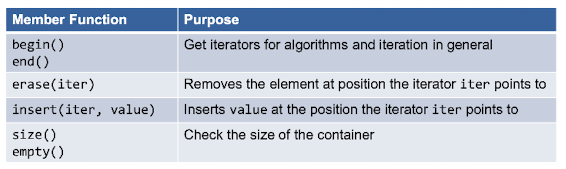
\includegraphics[width=0.75\linewidth]{container}
  \caption{Member Function of a Container}
\end{figure}

\subsection{Common Container Constructors}
\begin{lstlisting}[language=C++]
// Constructor with Initializer List
std::vector<int> v{1,2,3,5,6,11};
// Construction with a number of elements, five times a 42
std::list<int> l(5,42);
// Range with a pair of iterators
std::deque<int> q{begin(v), end(v)};
\end{lstlisting}

\subsection{Array}
C++'s std::array<T, N> is a fixed-size Container.  T is a template type parameter (= placeholder for type). N is a positive integer, template non-type parameter (= placeholder for a value). Elements can be accessed with a subscript operator [] or at(). The size is bound to the array object and can be queried using .size();. Avoid plain C-Array whenever possible: \lstinline[language=C++]|int arr[]{1, 2, 3, 4, 5};|
\begin{itemize}
  \itemsep -0.5em 
  \item at() throws an exception on invalid index access
  \item $[]$ has undefined behavior on invalid index access Behavior
  \item The size of an array must be known at compile-time and cannot be changed. Otherwise it contains N default-constructed elements: std::array<int, 5> emptyArray{};
\end{itemize}
\begin{center}
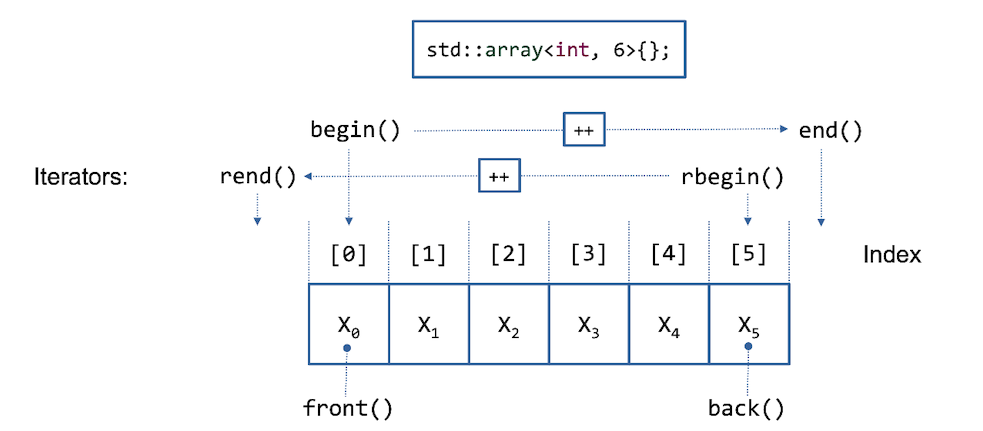
\includegraphics[width=0.75\linewidth]{images/array}
\end{center}

\subsection{Vector}
\begin{itemize}
  \itemsep -0.5em 
  \item C++'s std::vector<T> is a Container = contains its elements of type T (no need to allocate them).
  \item The elements are allocated on the heap.
  \item If a vector is passed to a function we can prevent a copy when we pass it as const.
\end{itemize}

\begin{center}
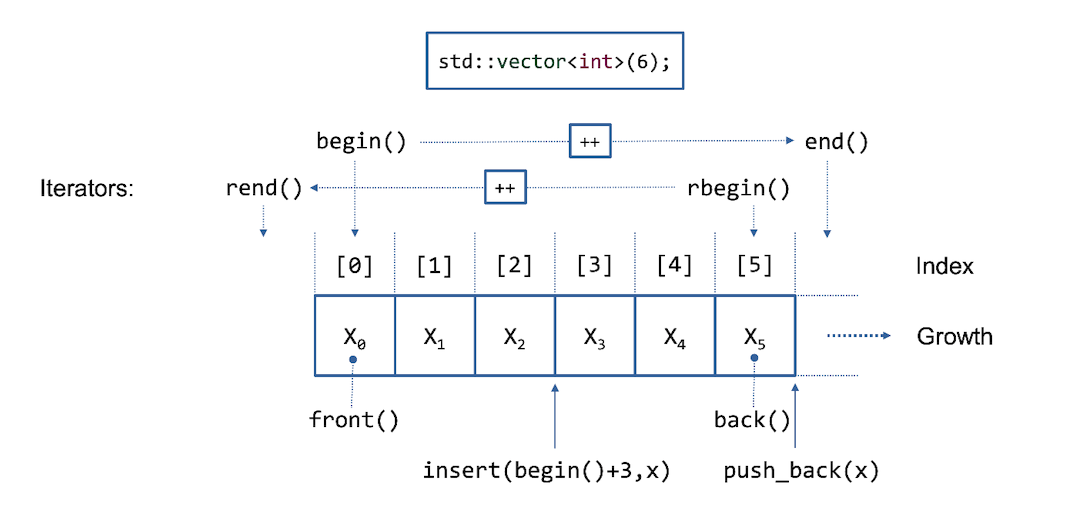
\includegraphics[width=0.75\linewidth]{images/vector}
\end{center}
\textbf{Append Elements to an std::vector<T>}
\begin{itemize}
  \itemsep -0.5em 
  \item \lstinline[language=C++]|v.push_back(<value>);|
  \item \lstinline[language=C++]|v.insert (<iterator-position>, <value>);|
\end{itemize}

\textbf{Filling a Vector with Values}
\begin{lstlisting}[language=C++]
std::vecor<int> v{};
v.resize(10);
std::fill(std::begin(v), std::end(v), 2);

std::vector<int> v(10); 
std::fill(std::begin(v), std::end(v), 2);

std::vector v(10, 2);

// Filling increased values with iota
std::vector<int> v(100); std:iota(std::begin(v), std::end(v), 1);
\end{lstlisting}

\textbf{Finding and counting elements of a vector} \\
 std::find() and std::find\_if() return an iterator to the first element that matches the value or condition.
\begin{lstlisting}[language=C++]
auto zero_it = std::find(std::begin(v), std::end(v), 0); if (zero_it == std::end(v)) {
std::cout << "no zero found \n"; }
\end{lstlisting}

\subsection{Double-Linked List}
\begin{itemize}
  \itemsep -0.5em 
  \item Very efficient inserting at any position.
  \item Lower efficiency in bulk operations.
  \item Only bi-directional iterators - no index access
\end{itemize}
\begin{figure}[h!]
  \centering
  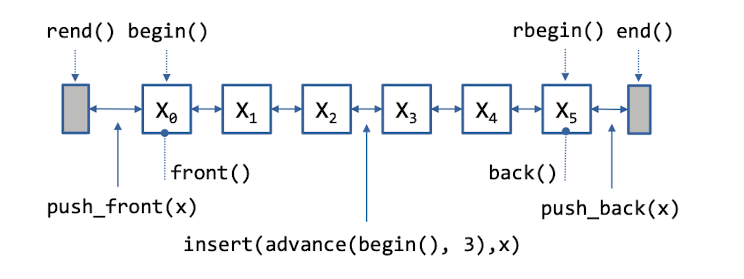
\includegraphics[width=0.6\linewidth]{list}
  \caption{Double-Linked List}
\end{figure}
\begin{lstlisting}[language=C++]
std::list<int> l = { 7, 5, 16, 8 };
l.push_front(25);
l.push_back(13);
// Insert an integer before 16 by searching
auto it = std::find(l.begin(), l.end(), 16);
if (it != l.end()) {
	l.insert(it, 42);
}
\end{lstlisting}

\subsection{Double-ended Queue, Deque}
Are like a vector, but additionally elements can be added efficiently to the start of the container.
\begin{figure}[h!]
  \centering
  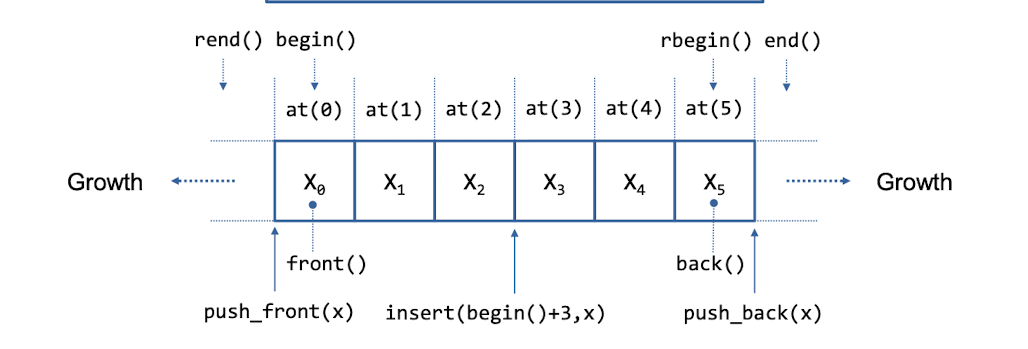
\includegraphics[width=0.75\linewidth]{deque}
  \caption{Deque}
\end{figure}

\subsection{Queue, FIFO Adapter}
In contrast to the Stack takes "pop()" the element from the begin of the Queue.
\begin{figure}[h!] 
  \centering
  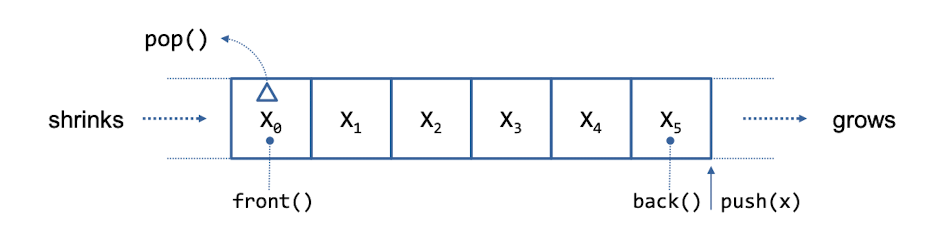
\includegraphics[width=0.75\linewidth]{queue}
  \caption{Queue}
\end{figure}
\begin{lstlisting}[language=C++]
std::queue<int> q{};
q.push(42);
std::cout << q.front();
q.pop();
\end{lstlisting}


\subsection{Stack, LIFO Adapter}
\begin{figure}[h!]
  \centering
  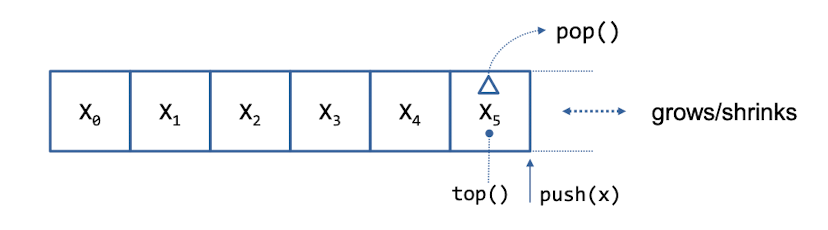
\includegraphics[width=0.75\linewidth]{stack}
  \caption{Stack}
\end{figure}

\subsection{Set}
The set does save all the elements in a tree. As a result there are no duplicates and all the elements are sorted automatically.
\begin{lstlisting}[language=C++]
#include <set>
std::set<int> s {7,1,4,3,2,5,6};

#include <string>
#include <algorithm> -> transform
#include <iostream> -> cout
#include <iterator> -> ostream_iterator
#include <cctype> -> lowercase

// insert
std::string const input{"test string"};
std::set<char> myset { };
std::transform(input.begin(), input.end(), inserter(myset, myset.begin()), [](char c) {
	return tolower(c);
});

// print
std::ostream_iterator<char> out {std::cout}
std::copy(myset.begin(), myset.end(), out};

\end{lstlisting}

\subsection{Multiset}
In contrast to the set does the multiset allow duplicates.
\begin{lstlisting}[language=C++]
#include <iostream>
#include <iterator>
#include <string>
#include <set>

using in=std::istream_iterator<std::string>;
using out=std::ostream_iterator<std::string>;
std::multiset<std::string> words{in{std::cin},in{}};
copy(cbegin(words), cend(words), out(std::cout, "\n"));
\end{lstlisting}

\subsection{Map}
In a map key-value pairs are stored, where the value can be in the set multiple times but the key is unique. Also the keys are stored in ascending order. The over can be overwritten with a 3rd template parameter.
\begin{figure}[h!]
  \centering
  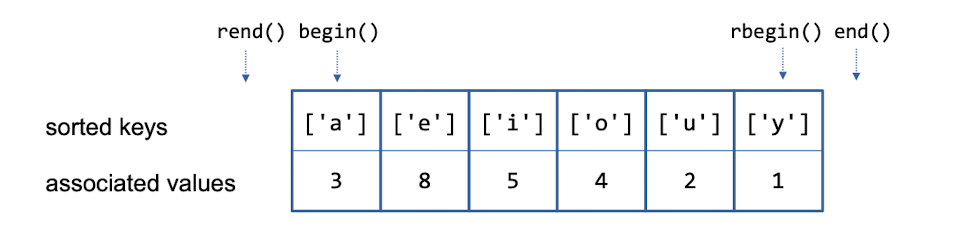
\includegraphics[width=0.75\linewidth]{map}
  \caption{Map}
\end{figure}
\begin{lstlisting}[language=C++]
std::map<char, size_t> vowels
{{'a',0},{'e',0},{'i',0},{'o',0},{'u',0},{'y',0}};

// Increment Value of Key
++vowels['a'];

// Beim Iterieren ist jedes Element ein pair<char, size>
for(auto const & p:vowels) {
	std::cout << p.first << " = "<< p.second << "\n";
}
\end{lstlisting}

\subsection{Multimap}
Allows to have multiple keys.
